
We focus on exact support recovery problems in this chapter, and generalize the results we obtained in Chapter \ref{chap:phase-transitions} to additive error models with much relaxed distributional and dependence assumptions.  
Sufficient conditions for exact support recovery \eqref{eq:exact-recovery} are given in 
Section \ref{subsec:sufficient}.  A very general class of dependence structures characterized by the uniform relative stability concept will 
be introduced in Section \ref{subsec:URS}, to prepare us for the necessary condition in Section \ref{subsec:necessary}.
Section \ref{subsec:dense-signals} discusses the dense signal regime, and Section \ref{suppsec:numerical} illustrates the phase transition 
phenomena with numerical examples.  We begin with an overview of our results in the context of the existing literature.




\section{Contributions and related work} Consider the additive error model \eqref{eq:model-additive} with the triangular array of errors,
\begin{equation} \label{eq:error-array}
    {\cal E} = \left\{ (\epsilon_p(i))_{i=1}^p,\ p=1,2,\dots\right\},
\end{equation}
where the $\epsilon_p(i)$'s have common cumulative distribution function $F(x)=\P[\epsilon_p(i)\le x]$.
In contrast to the assumptions in Chapter \ref{chap:phase-transitions}, we only require the errors to have common marginal distributions, and allow them to have potentially arbitrary dependence.
% We will study the role of dependence in support recovery problems in Section \ref{sec:URS}. 
 

Although our method of analysis applies to all light-tailed error distributions with rapidly varying tails (see Definition \ref{def:rapid-variation}), to be concrete and better convey the main ideas, we will focus on the class of $\mathrm{AGG}(\nu)$ laws (see Definition \ref{def:AGG}).
Extensions of the results to other error models are presented in Section \ref{suppsec:other-boundaries}.

As in Chapter \ref{chap:phase-transitions}, we assume the signals in model \eqref{eq:model-additive} to be a sparse vector $\mu = \left(\mu(i)\right)_{i=1}^p$ where the sparsity, with a few exceptions which will be explicitly stated, is parametrized as
\begin{equation} \label{eq:sparsity-parametrized}
    s = |S_p| = \lfloor p^{1 -\beta} \rfloor, % \quad \text{with } 0 < \beta \le 1 \; \text{(fixed)},
\end{equation}
with $0 < \beta \le 1$ fixed.

We assume that the non-zero entries of $\mu$ are positive and take values in the interval $\left[\underline{\Delta},\overline{\Delta}\right)\subset (0,\infty)$.
That is, $0<\underline{\Delta}\le\mu(i)<\overline{\Delta}\le+\infty$, for all $i\in S_p$.
The lower and upper bound on the signal sizes $\underline{\Delta}$ and $\overline{\Delta}$ are parametrized as
\begin{equation} \label{eq:signal-size-parametrized}
    \underline{\Delta} = \underline{\Delta}(p) = (\nu \underline{r} \log{p})^{1/\nu} \quad \text{and} \quad
    \overline{\Delta} = \overline{\Delta}(p)  = (\nu \overline{r} \log{p})^{1/\nu},
\end{equation}
with parameters $0 < \underline{r} \le \overline{r} \le +\infty$.
Notice that the parametrization now depends on the shape of the assumed error distributions $\mathrm{AGG}(\nu)$ through the parameter $\nu$.

According to Lemma \ref{lemma:risk-exact-recovery-probability}, in order to study the asymptotic behaviors of $\mathrm{risk}^{\mathrm{E}}$, it is sufficient to establish minimal conditions under which the support sets can be consistently estimated, i.e.,
\begin{equation} \label{eq:exact-recovery} 
    \P[\widehat{S}_p = S_p] \longrightarrow 1 \quad \text{as } \; p\to\infty, 
\end{equation}
where $\widehat{S}_p$ is an estimate of the true signal support set $S_p$.

\medskip

Several authors have studied the support recovery problem in terms of the Hamming loss and obtained minimax optimality results (see, e.g., \cite{ji2012ups, genovese2012comparison, jin2014optimality, butucea2018variable}).
% We briefly review the recent work by \cite{butucea2018variable}, whose .
In the special case of Gaussian marginals, \cite{butucea2018variable} showed that the boundary \eqref{eq:strong-classification-boundary-Gaussian} exists in a minimax sense.
That is, when the errors are \emph{independent} Gaussians, the Hamming loss cannot be made to vanish if the signal sizes fall below the boundary \eqref{eq:strong-classification-boundary-Gaussian} by any procedure. 
Conversely, if signal size falls below, the Hamming loss can be made to vanish with a specific thresholding procedure.

Unfortunately, as pointed out in Section \ref{sec:risks-relations}, vanishing Hamming loss is only sufficient, not necessary for support recovery \eqref{eq:exact-recovery}, and the latter sharp results do not carry over directly to the study of the probability of support recovery or exact support recovery risk.
More importantly, despite their elegance, these Hamming loss-minimax studies naturally reduce to the analysis of the elementary case of iid data, and is by design blind to non-trivial error-dependence structures.
This prevents us from fully exploring of the phase transition phenomena under other dependence conditions.
% This is arguably a consequence of the inherent limitation of the Hamming-loss approach. 
% For practitioners, a minimax statement in the Gaussian case seems to offer little guidance.
% Indeed, in applications, independence is an exception rather than the rule; Gaussianity of the errors may also be unnecessarily restrictive.

So far in the literature, the role of dependence, and that of the distributional assumptions in model 
\eqref{eq:model-additive} have remained largely unexplored.  This chapter offers advances in both directions, and provides a close-to-complete solution of the exact support recovery problem. (See also, Chapter \ref{chap:URS}.)
We briefly summarize our contributions next.


\medskip
In Section \ref{subsec:sufficient}, we study exact support recovery in the sense of \eqref{eq:exact-recovery} directly, under general 
distributional and dependence assumptions.  In particular, we describe the phase transition phenomena in the dependent AGG model, under the scaling described in \eqref{eq:sparsity-parametrized} and \eqref{eq:signal-size-parametrized}.
Consider the function
\begin{equation} \label{eq:strong-classification-boundary}
    g(\beta) = g_\nu(\beta) = (1 + (1 - \beta)^{1/\nu})^\nu, \quad \nu>0,
\end{equation}
which we refer to as the {\em strong classification boundary}.
In Theorem \ref{thm:sufficient} we show that, 
% under the general distributional assumptions in Section \ref{subsec:set-up}, 
if the signal sizes are above the boundary (i.e., $\underline{r}> g(\beta)$), the \ac{FWER}-controlling procedures described in Section \ref{sec:statistical-procedures} with appropriately calibrated levels achieve \emph{exact support recovery} as in \eqref{eq:exact-recovery}.

Conversely, we show in Theorem \ref{thm:necessary}, that for a surprisingly large class of dependence structures characterized by the concept of \emph{uniform relative stability} (URS, see Definition \ref{def:URS} below), when the signal size is below the boundary  (i.e., $r<g(\beta)$), no thresholding procedure can achieve the asymptotically perfect support recovery \eqref{eq:exact-recovery}. In fact,
\begin{equation} \label{eq:exact-recovery-failure}
    \mathbb{P}\left[\widehat{S}_p=S_p\right]\longrightarrow 0,\quad \mbox{ as }p\to \infty,
\end{equation}
for all $\widehat{S}_p$ in the form of \eqref{eq:thresholding-procedure}.

These two results show that the thresholding procedures obey a phase transition phenomenon in a strong, \emph{point-wise} sense over the class of URS dependence structures, and over the class of AGG$(\nu),\ \nu>0$ error distributions. 
The conclusions are fundamentally stronger and more informative than the minimax statements in the literature (see, e.g., \cite{butucea2018variable}).
The techniques developed in this here are also entirely different from those in \citet{ji2012ups} or \citet{butucea2018variable}, and transparent characterizations of the dependence conditions under which the phase transition type result holds will be established in the Chapter \ref{chap:URS} later.

%In Chapter \ref{sec:optimality} we study the finite-sample optimality of the threshold-based support estimation procedures in a Bayesian setting. 

% The strong classification boundary $g$ characterizes a phase-transition phenomenon similar to that of the signal detection and approximate support recovery. 
% A preview of this result is presented in Figure \ref{fig:phase}.

% \begin{figure}
%       \centering
%       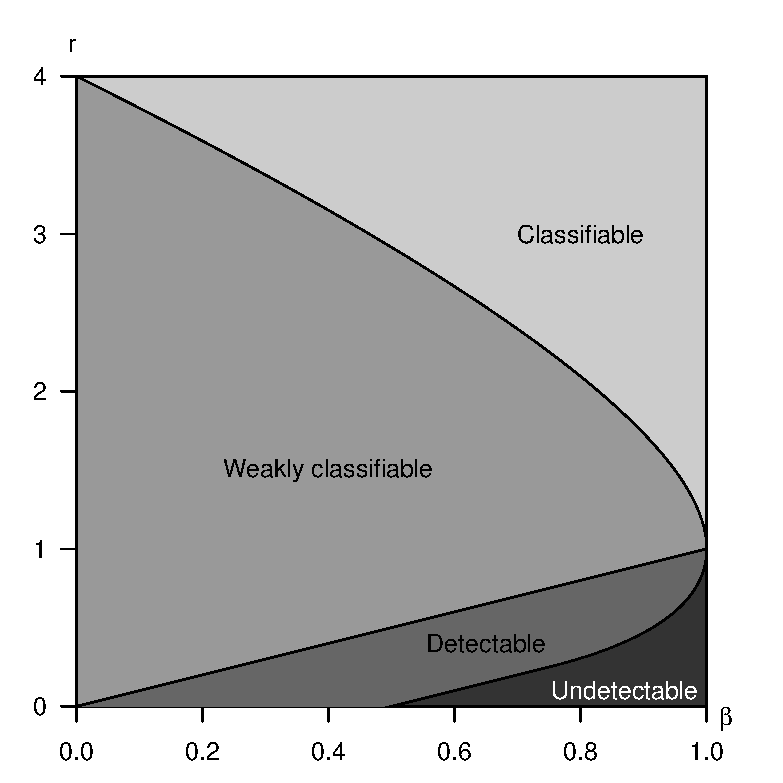
\includegraphics[width=0.45\textwidth]{./figures/phase_diagram_Gaussian_no_dashed_area.eps}
%       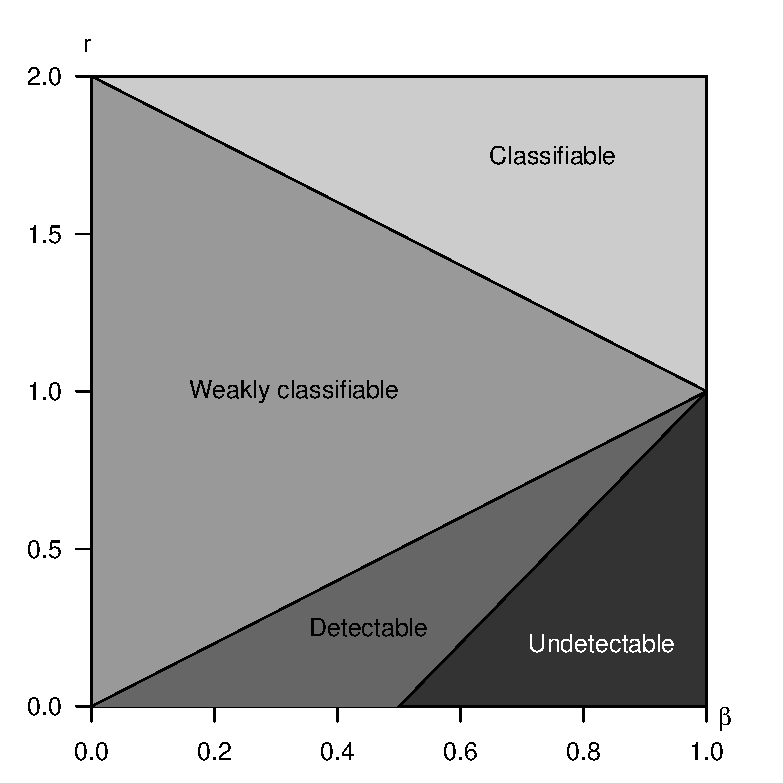
\includegraphics[width=0.45\textwidth]{./figures/phase_diagram_double_exponential.eps}
%       \caption{The phase diagrams of the detection, weak classification, and strong classification boundaries against sparse alternatives under Gaussian (left) and Laplace distributed (right) errors. Here $\beta$ and ${r}$ parametrize the signal sparsity and the lower and upper bounds of the signal sizes, respectively. 
%       The signal detection problem can be answered perfectly (asymptotically) inside the \emph{Detectable} region; false discovery proportion and non-discovery proportion can be made to vanish in the \emph{Weakly classifiable} region. We study in this paper the strong classification boundary, above which the support recovery can be achieved \emph{exactly} in the \emph{Classifiable} region $\{(\beta, {r}):{r}>g(\beta)\}$. 
%       In a large class of dependence structures characterized by URS, when signal sizes fall below the strong classification boundary \eqref{eq:strong-classification-boundary}, i.e. $\{(\beta, {r}):{r}<g(\beta)\}$, no thresholding procedure succeeds in the exact support recovery problem. }
%       \label{fig:phase}
% \end{figure}


\medskip
The phase transition phenomena for two additional classes of error distributions with either heavier or lighter tails than the AGG distributions will be described in Section \ref{suppsec:other-boundaries}.

\medskip
To conclude this summary, we emphasize that the sharp phase transition results established in this chapter apply only to
the general class of thresholding procedures.  In Chapter \ref{chap:optimality}, we characterize the finite-sample Bayes optimal support estimation procedures.
It will turn out that in many cases the optimal procedures are in fact thresholding procedures.  This will lead to complete phase transition
results valid for all types of support estimators, for certain classes of error models. In general, however, thresholding procedures
can be sub-optimal.  This has only recently been noticed by the statistical community in the case when the errors have heavy (regularly-varying) tails. 
\citet{arias2019detection} discussed the phenomenon in approximate support recovery problems.  In this case, we also demonstrate the absence 
of a phase transition phenomenon in exact support recovery by thresholding, in Section \ref{suppsec:heavy-tailed}. 


% In this sense, for $\nu\ge 1$ our results are rather complete.  We note here that our focus is not on minimax analysis of the support recovery problem, where a large class of distributional and dependence structures are considered.  
% In some sense, the worst case scenario (see also \cite{butucea2018variable}) is when the errors are independent.  
% In contrast, we establish the phase-transition phenomenon, for fixed but very general dependence conditions characterized by the URS property.


%We show that when the error-distribution $F$ is log-concave, then the thresholding procedures are optimal (for independent errors).  Therefore, in this regime the {\em strong classification boundary} $g$ is universal.  
%That is, if $r<g(\beta)$, no estimator can achieve perfect support recovery as $p\to\infty$. 
% \fbox{maybe skip the next sentence} 
% In fact, going beyond the class of rapidly varying distributions, (e.g., for heavy Pareto-type tails) the support recovery problem is fundamentally different and there may no longer be a phase-transition phenomenon.


%\section{Exact support recovery under AGG errors}
%\label{sec:boundary}

% We present the sufficient conditions for asymptotic exact support recovery in Section \ref{subsec:sufficient}.
% The study of maxima plays a central part in the study of support recovery problems.
% We present the key concepts regarding the behavior of the maxima, and in particular, the concentration of maxima phenomena, in Sections \ref{subsec:RS} and \ref{subsec:URS}. 
% These concepts enable to state a partial converse in Section \ref{subsec:necessary}.


\section{Sufficient conditions for exact support recovery}
\label{subsec:sufficient}

Following \citet*{butucea2018variable}, we define the parameter space for the signals $\mu$ as
\begin{align} \label{eq:minimax-signal-config-over}
    \Theta_p^+(\beta, \underline{r}) &= \{\mu\in\mathbb{R}^p:\;\text{there exists a set }S_p\subseteq\{1,\ldots,p\}\;\text{ such that }|S_p|\le\lfloor p^{1-\beta}\rfloor, \nonumber \\
    &\quad\quad\mu(i)\ge (\nu\underline{r}\log{p})^{1/\nu}\;\text{for all }i\in S_p,\;\text{and }\mu(i)=0\;\text{for all }i\not\in S_p\}.
\end{align}
Our first result states that, when $F\in \text{AGG}(\nu)$ with $\nu>0$, regardless of the error dependence structure, (asymptotic) perfect support recovery is achieved by applying Bonferroni's procedure with appropriately calibrated FWER, as long as the minimum signal size $\underline{r}$ is above the strong classification boundary \eqref{eq:strong-classification-boundary}.

\begin{theorem} \label{thm:sufficient}
Let the errors have common marginal distribution $F\in \text{AGG}(\nu)$ with $\nu>0$.
Let $\widehat{S}_p$ be the Bonferroni's procedure \eqref{eq:Bonferroni-procedure} with vanishing FWER $\alpha = \alpha(p) \to 0$, such that %\fbox{slower than any polynomial}
$\alpha p^\delta\to \infty$ for every $\delta>0$.
If
\begin{equation} \label{eq:signal-above-boundary}
    \underline{r} > f_{\mathrm{E}}(\beta) = (1 + (1 - \beta)^{1/\nu})^\nu,
\end{equation}
then we have
\begin{equation} \label{eq:exact-supporot-recovery}
    \lim_{p\to\infty}\sup_{\mu\in\Theta_p^+(\beta, \underline{r})} \P[\widehat{S}_p \neq S_p] = 0.
\end{equation}
\end{theorem}
\begin{proof}%[Proof of Theorem \ref{thm:sufficient}]
Throughout the proof, the dependence on $p$ will be suppressed to simplify notations when such omissions do not lead to ambiguity.

Under the $\text{AGG}(\nu)$ model, it is easy to see from equation \eqref{eq:AGG-quantiles} that the thresholds in Bonferroni's procedure are 
\begin{equation}\label{e:AGG-threshold}
t_p = F^{\leftarrow}(1 - \alpha/p) = (\nu\log{(p/\alpha)})^{1/\nu}(1+o(1)).
\end{equation}
It is known that Bonferroni's procedure $\widehat{S}_p = \left\{i:x(i)>t_p\right\}$ controls the FWER.  Indeed,
\begin{align} \label{eq:Bonferroni-FWER-control}
    \P\left[\widehat{S} \subseteq S\right] 
        &= 1 - \P\left[\max_{i\in S^c}x(i) > t_p\right] = 1 - \P\left[\max_{i\in S^c}\epsilon(i) > t_p\right]\nonumber \\
      % \ge 1 - \P\left[\max_{i\in\{1,\ldots,p\}}\epsilon(i) > t_p\right] \nonumber \\
        &\ge 1 - \sum_{i=1}^{p}\P\left[\epsilon(i)>t_p\right] \ge 1 - \alpha(p) \to 1,
\end{align}
where we used the union bound in the first inequality. 
Notice that the lower bound \eqref{eq:Bonferroni-FWER-control} is independent of the parameter $\mu$ (as well as the dependence structures), and hence holds uniformly over the parameter space, i.e.,
\begin{equation} \label{eq:exact-supporot-recovery-FWER}
    \lim_{p\to\infty}\inf_{\mu\in\Theta_p^+(\beta, \underline{r})} P[\widehat{S}_p \subseteq S_p] = 1.
\end{equation}


On the other hand, for the probability of no missed detection, we have:
\begin{equation*}
    \P\left[\widehat{S} \supseteq S\right] 
        = \P\left[\min_{i\in S}x(i) > t_p\right]
        = \P\left[\min_{i\in S}x(i) - (\nu\underline{r}\log p)^{1/\nu} > t_p - (\nu\underline{r}\log p)^{1/\nu} \right].
\end{equation*}
Since the signal sizes are no smaller than $(\nu\underline{r}\log p)^{1/\nu}$, we have
\begin{equation*}
    x(i) - \left(\nu\underline{r}\log{p}\right)^{1/\nu} \ge \epsilon(i), \quad \text{for all }i\in S,
\end{equation*}
and hence we obtain
\begin{equation} \label{eq:sufficient-proof-eq1}
    \P\left[\widehat{S} \supseteq S\right] \ge 
    \P\left[\min_{i\in S}\epsilon(i) > (\nu\log{(p/\alpha)})^{1/\nu}(1+o(1)) - (\nu\underline{r}\log p)^{1/\nu} \right],
\end{equation}
where we plugged in the expression for $t_p$ in \eqref{e:AGG-threshold}.
Now, since the minimum signal size is bounded below by $\underline{r} > \left(1 + (1-\beta)^{1/\nu}\right)^\nu$, we have $\underline{r}^{1/\nu}-(1-\beta)^{1/\nu}>1$, and so we can pick a $\delta > 0$ such that 
\begin{equation} \label{eq:choice-of-delta}
    \delta < \left(\underline{r}^{1/\nu} - (1-\beta)^{1/\nu}\right)^\nu - 1.
\end{equation}
Since by assumption, for all $\delta>0$, we have $p^{-\delta} = o\left(\alpha(p)\right)$, there is an
$M=M(\delta)$ such that $p/\alpha(p) < p^{1+\delta}$ for all $p\ge M$. Thus, from \eqref{eq:sufficient-proof-eq1}, we further conclude that for $p\ge M$ we have
\begin{align}
    \P\Big[\widehat{S} \supseteq S\Big]
      &\ge \P\Big[\min_{i\in S}\epsilon(i) > \left((1+\delta)\nu\log{p}\right)^{1/\nu}(1+o(1)) - (\nu\underline{r}\log p)^{1/\nu} \Big] \nonumber \\
      &= \P\Big[\max_{i\in S}\left(-\epsilon(i)\right) < \underbrace{\left(\underline{r}^{1/\nu} - (1+\delta)^{1/\nu}\right)(\nu\log{p})^{1/\nu}(1+o(1))}_{=:\text{A}} \Big] \nonumber \\
      &\ge 1 - \lfloor p^{1-\beta} \rfloor \times \overline{F}_-(\text{A}), \label{eq:sufficient-proof-eq2}
      % &\ge 1 - |S|\times\P\Big[(-\epsilon(1)) \ge \left(\underline{r}^{1/\nu} - (1+\delta)^{1/\nu}\right)(\nu\log{p})^{1/\nu}(1+o(1)) \Big] 
\end{align}
where $\overline{F}_-(x) = \P[-\epsilon(i)>x]$ is the survival function of the $(-\epsilon(i))$'s.
Notice that \eqref{eq:sufficient-proof-eq2} follows from the union bound and the assumption that ${|S_p|}\le{\lfloor p^{1-\beta}\rfloor}$. 
Therefore, the lower bound does not depend on $\mu$ (nor on the error dependence structure), and holds uniformly in the parameter space. In turn, we obtain 
\begin{equation} \label{eq:exact-supporot-recovery-FWNR}
    \inf_{\mu\in\Theta_p^+(\beta, \underline{r})} \P[\widehat{S}_p \supseteq S_p] \ge 1 - \lfloor p^{1-\beta} \rfloor \times \overline{F}_-(\text{A}).
\end{equation}

If $\beta=1$, we conclude that the right-hand-side of \eqref{eq:exact-supporot-recovery-FWNR} 
converges to $1$, since $\text{A}\to+\infty$.

Let now $\beta\in (0,1)$ and $u_p^- :=  F_-^{\leftarrow}(1-1/p)$. 
The fact that $p\overline{F}_-(u_p^-) \le 1$, implies
\begin{equation}
    \lfloor p^{1-\beta} \rfloor \times \overline{F}_-(\text{A}) \le 
    \frac{\overline{F}_-\left(\text{B}\times{u_{\lfloor p^{1-\beta}\rfloor}^-}\right)} {\overline{F}_-\left({u_{\lfloor p^{1-\beta}\rfloor}^-}\right)} \label{eq:sufficient-proof-eq3}
    % \P\Big[\frac{\max_{i\in S}(-\epsilon(i))}{u_{|S|}}\frac{u_{|S|}}{u_{\lfloor p^{1-\beta}\rfloor}} < \underbrace{\frac{\underline{r}^{1/\nu} - (1+\delta)^{1/\nu}}{(1-\beta)^{1/\nu}}\left(1+o(1)\right)}_{=:\text{B}}\Big], \label{eq:exact-supporot-recovery-FWNR}
\end{equation}
where $\text{B} := {\text{A}}/{u_{\lfloor p^{1-\beta}\rfloor}^-}$.

Notice that by assumption, the $-\epsilon(i)$'s are also 
AGG$(\nu)$ distributed and by Proposition \ref{prop:quantile}, 
$u_p^{-}:= F_-^{\leftarrow}(1-1/p) \sim (\nu \log(p))^{1/\nu}$,
as $p\to\infty$. Therefore, we have
\begin{equation} \label{eq:sufficient-proof-eq4}
    u_{\lfloor p^{1-\beta}\rfloor}^- \sim \left(\nu(1-\beta)\log{p}\right)^{1/\nu}
\end{equation}
and 
\begin{equation*}
\text{B} = \frac{\text{A}}{u_{\lfloor p^{1-\beta}\rfloor}^-}
= \frac{\underline{r}^{1/\nu} - (1+\delta)^{1/\nu}}{(1-\beta)^{1/\nu}}\left(1+o(1)\right) \to c>1
\end{equation*}
as $p\to\infty$, by our choice of $\delta$ in \eqref{eq:choice-of-delta}.

Finally, since the distribution $F_-$ has \emph{rapidly varying} tails (by Definition \ref{def:rapid-variation} and Example \ref{exmp:AGG}), applying Proposition \ref{prop:rapid-varying-tails}, we conclude that \eqref{eq:sufficient-proof-eq3} vanishes. Consequently, the lower bound on the right-hand-side of \eqref{eq:exact-supporot-recovery-FWNR} converges to 1.
This, combined with \eqref{eq:exact-supporot-recovery-FWER}, entails {$\lim_{p\to\infty} \inf_{\mu\in\Theta_p^+(\beta, \underline{r})} \P[\widehat{S}_p = S_p]= 1$, and hence the desired conclusion \eqref{eq:exact-supporot-recovery}, which completes the proof}.
\end{proof}

\medskip
We end this section with several comments and applications of Theorem \ref{thm:sufficient}.
\begin{corollary}[Classes of procedures attaining the boundary]
\label{cor:FWER-controlling_procedures}  
Relation \eqref{eq:exact-supporot-recovery} holds for any FWER-controlling procedure that is strictly more powerful than Bonferroni's procedure. 
This includes Holm's procedure \citep*{holm1979simple}, and in the case of independent errors, Hochberg's procedure \citep*{hochberg1988sharper}, and the {\v{S}}id{\'a}k procedure \citep*{vsidak1967rectangular}.
\end{corollary}

\begin{example} \label{exmp:FWER-controlling_procedures}
Under Gaussian errors, the particular choice of the thresholding at $t_p = \sqrt{2\log{p}}$ in \eqref{eq:Bonferroni-procedure} corresponds to a Bonferroni's procedure with FWER decreasing at a rate of ${\cal O}((\log{p})^{-1/2})$, and hence Theorem \ref{thm:sufficient} applies. 
By Corollary \ref{cor:FWER-controlling_procedures}, Holm's procedure --- and when the errors are independent, the {\v{S}}id{\'a}k, and Hochberg procedures --- with FWER controlled at $(\log{p})^{-1/2}$ all achieve perfect support recovery provided that $\underline{r}>f_{\mathrm{E}}(\beta)$.

\begin{proof}[Example \ref{exmp:FWER-controlling_procedures}]
By the Mill's ratio for the standard Gaussian distribution,
$$
\frac{t_p \P\left[Z>t_p\right]}{\phi(t_p)} \to 1,\quad \text{as}\quad t_p\to\infty,
$$
where $Z\sim \text{N}(0,1)$. 
Using the expression for $t_p = \sqrt{2\log{p}}$, we have
$$
p \;\P\left[Z>t_p\right] \sim \sqrt{2\pi}^{-1}\left(2\log{p}\right)^{-1/2} \to 0,
$$
as desired. The rest of the claims follow from Corollary \ref{cor:FWER-controlling_procedures}.
\end{proof}
\end{example}


The statements in Theorem \ref{thm:sufficient} can be strengthened, to prepare us for a minimax result given in Section \ref{sec:minimax} below.

\begin{remark} \label{rmk:sufficient-strengthened}
In the proof of Theorem \ref{thm:sufficient}, both \eqref{eq:Bonferroni-FWER-control} and \eqref{eq:sufficient-proof-eq2} hold uniformly over all error dependence structures.
Therefore, \eqref{eq:exact-supporot-recovery-FWER} and \eqref{eq:exact-supporot-recovery-FWNR} may be strengthened to yield
\begin{equation} \label{eq:exact-supporot-recovery-strengthened}
    \lim_{p\to\infty}\sup_{\substack{\mu\in\Theta_p^+(\beta, \underline{r})\\ {\cal E}\in D(F)}} P[\widehat{S}_p \neq S_p] = 0,
\end{equation}
for $\underline{r} > f_{\mathrm{E}}(\beta)$, where $D(F)$ is the collection of all arrays with common marginal $F$, i.e., 
\begin{equation} \label{eq:common-marginal-distribution}
    D(F)=\{{\cal E}=(\epsilon_p(i))_p:\;\epsilon_p(i)\sim F\;\text{for all }i=1,\ldots,p, \text{and}\; p=1,2,\ldots\}.
\end{equation}
\end{remark}

\begin{remark}
We emphasize that Theorem \ref{thm:sufficient} holds for errors with \emph{arbitrary} dependence structures. 
Intuitively, this is because the maxima of the errors grow at their fastest in the case of independence (recall Remark \ref{rem:iid-max}). 
Formally, the light-tailed nature of the error distribution allowed us to obtain sharp tail estimates via simple union bounds, 
valid under arbitrary dependence.
% Formally, this result stems from the fact that maxima of distributions with \emph{rapidly varying tails} (Definition \ref{def:rapid-variation}) can be bounded from above using quantiles of their marginal distribution, under arbitrary dependence.
\end{remark}
% We turn next to the study of maxima and present the tools used in the proof of Theorem \ref{thm:sufficient}.
% Thus, the support recovery problem is hardest under independent errors.
% The relationship between dependence and the behavior of maxima is discussed next in Section \ref{sec:URS}, where we will see that the phase-transition phenomenon is not limited to just the AGG models and independent errors; such phenomenon exists for all error models with rapidly varying tails, and under a surprisingly large class of dependent structures.
% On the other hand, the converse of Theorem \ref{thm:sufficient} will need an (extremely mild) assumption on error dependence structures.


\section{Dependence and uniform relative stability}
\label{subsec:URS}

An important ingredient needed for a converse of Theorem \ref{thm:sufficient} is an appropriate characterization of the error dependence structure under which the strong classification boundary \eqref{eq:strong-classification-boundary} is tight.
The notion of \emph{uniform relative stability} turns out to be the key.
% in characterizing such dependence structures when studying the behavior of maxima of dependent light-tailed sequences.

\begin{definition}[Uniform Relative Stability] \label{def:URS}
Under the notations established in Definition \ref{def:RS}, the triangular array ${\cal E}$ is said to have uniform relatively stable (URS) maxima if for \emph{every} sequence of subsets $S_p\subseteq\{1,\ldots,p\}$ such that $|S_p| \to \infty$, we have
\begin{equation} \label{eq:URS-condition}
    \frac{1}{u_{|S_p|}} M_{S_p} := \frac{1}{u_{|S_p|}} \max_{i\in S_p} \epsilon_p(i) \xrightarrow{\P} 1,
\end{equation}
as $p\to\infty$, where $u_q,\ q\in \{1,\ldots,p\}$ is the generalized quantile in \eqref{eq:quantiles}.
The collection of arrays ${\cal E} = \{ \epsilon_p(i) \}$ with URS maxima is 
denoted $U(F)$.
\end{definition}

Uniform relative stability is, as its name suggests, a stronger requirement on dependence than relative stability (recall Definition \ref{def:RS}). 
Proposition \ref{prop:rapid-varying-tails} states that an array with iid components sharing a marginal distribution $F$ with rapidly varying tails (Definition  \ref{def:rapid-variation}) has relatively stable maxima; it is easy to see that URS also follows, by independence of the entries.

\begin{corollary} \label{cor:AGG-is-URS}
An independent array ${\cal E}$ with common marginals $F\in\text{AGG}(\nu)$, $\nu>0$, is URS; in this case, URS holds with $u_{|S_p|} \sim \left(\nu\log{|S_p|}\right)^{1/\nu}$.
\end{corollary}

On the other hand, RS and URS hold under much broader dependence structures than just 
independent errors. 
These conditions are extremely mild and can be shown to hold for many classes of error models.  
In Chapter \ref{chap:URS}, we will focus extensively on the Gaussian case, which is of great interest in applications and is rather challenging. 
We will provide simple necessary and sufficient condition for uniform relative stability in terms of the covariance structures.

The relative stability concepts are important because they characterize the dependence structures under which the maxima of error sequences {\em concentrate} around the quantiles \eqref{eq:quantiles} in the sense of \eqref{eq:RS-condition}.
This concentration of maxima phenomena, in turn, is the key to establishing the necessary conditions of the phase transition results in support recovery problems.

% The importance of the URS dependence class in statistics is seen in the study of support recovery problems, discussed next.

\section{Necessary conditions for exact support recovery}
\label{subsec:necessary}

With the preparations from Section \ref{subsec:URS}, we are ready to state the necessary conditions for exact support recovery \eqref{eq:exact-recovery} by thresholding procedures. 
It turns out that the strong classification boundary \eqref{eq:strong-classification-boundary} is tight, under the general dependence structure characterized by URS (Definition \ref{def:URS}).

Formally, we define the parameter space for the signals $\mu$ to be
\begin{align} \label{eq:minimax-signal-config-under}
    \Theta_p^-(\beta, \overline{r}) &= \{\mu\in\mathbb{R}^p:\;\text{there exists a set }S_p\subseteq\{1,\ldots,p\}\;\text{ such that }|S_p|=\lfloor p^{1-\beta}\rfloor, \nonumber \\
    &\quad\quad0<\mu(i)\le(\nu\overline{r}\log{p})^{1/\nu}\;\text{for all }i\in S_p,\;\text{and }\mu(i)=0\;\text{for all }i\not\in S_p\}.
\end{align}


\begin{theorem} \label{thm:necessary}
    Let ${\cal E}$ be a triangular array with common $\text{AGG}(\nu)$ marginal $F$, $\nu > 0$.
    % Let the signal $\mu$ have $|S_p| = \lfloor p^{(1-\beta)} \rfloor$ non-zero entries where $\beta\in(0,1]$, where the signal sizes $\mu(i)$, $i\in S_p$ are at most $\overline{\Delta} = \left(\nu\overline{r}\log p\right)^{1/\nu}$.
    % and the signals $\mu$ have $s=|S|=\lfloor p^{1-\beta}\rfloor$ be as described in Theorem \ref{thm:sufficient}. 
    Assume further that the errors ${\cal E}$ have uniform relatively stable maxima and minima, i.e., ${\cal E}\in U(F)$, and $(-{\cal E}) = \{-\epsilon_{p}(i)\} \in U(F)$.
    If 
    \begin{equation} \label{eq:signal-below-boundary}
        \overline{r} < f_{\mathrm{E}}(\beta) = \left(1+(1-\beta)^{1/\nu}\right)^\nu,
    \end{equation}
    then
    \begin{equation} \label{eq:classification-impossible-dependent}
        \lim_{p\to\infty} \inf_{\widehat{S}_p\in{\cal T}} \inf_{\mu\in{\Theta_p^-(\beta, \overline{r})}} \P[\widehat{S}_p \neq S_p] = 1,
    \end{equation}
    where ${\cal T}$ is the class of all thresholding procedures \eqref{eq:thresholding-procedure}.
\end{theorem}
\begin{proof} %[Proof of Theorem \ref{thm:necessary}]
To avoid cumbersome double subscript notations, we will sometimes suppress dependence on $p$ of the set sequences $\widehat{S}_p$ and $S_p$ in the proof.

Since the estimator $\widehat{S}_p = \{x(i) \ge t_p(x)\}$ is thresholding, exact support recovery takes place if and only if the threshold separates the signals and null part, i.e.,
\begin{equation*}
    \P[\widehat{S}_p = S_p] 
    = \P\left[\max_{i\in S^c}x(i) < t_p(x) \le \min_{i\in S}x(i)\right]
    \le \P\left[\max_{i\in S^c}x(i) < \min_{i\in S}x(i)\right].
\end{equation*}
Since the right-hand-side does not depend on the procedure $\widehat{S}_p$, we also have
\begin{equation} \label{eq:classification-possible-dependent-proof-1}
    \sup_{\widehat{S}_p\in{\cal T}} \P[\widehat{S}_p = S_p] 
    \le \P\left[\max_{i\in S^c}x(i) < \min_{i\in S}x(i)\right]
    \le \P\left[{\max_{i\in S^c}\epsilon(i)} < {\overline{\Delta} + \min_{i\in S}\epsilon(i)}\right],
\end{equation}
where we used the assumption that the signal sizes are no greater than $\overline{\Delta}$.
Let $S^* = S_p^*$ be a sequence of support sets that maximize the right-hand-side of \eqref{eq:classification-possible-dependent-proof-1}, i.e., let
$$
S_p^* = \argmax_{S\subseteq\{1,\ldots,p\}:|S| = \lfloor p^{1-\beta}\rfloor} \P\left[{\max_{i\in S^c}\epsilon(i)} < {\overline{\Delta} + \min_{i\in S}\epsilon(i)}\right],
$$
where ties can be broken lexicographically if multiple maximizers exist.
Then,
% Since there is only a finite number support set $S$ in $\mathcal{S} = \left\{S\subseteq\{1,\ldots,p\};|S|=\lfloor p^{1-\beta}\rfloor\right\}$, we can bound \eqref{eq:classification-possible-dependent-proof-1} from above uniformly over $\mathcal{S}$ as well.
% In particular, let 
% $$
% S^* = S^*_p \in \argmax_{S\in{\mathcal{S}}}\P\left[{\max_{i\in S^c}\epsilon(i)} < {\overline{\Delta} + \min_{i\in S}\epsilon(i)}\right],
% $$
we obtain the following bound which only depends on $\overline{r}$ and the distribution of ${\cal E}$,
\begin{align}
    \sup_{\widehat{S}_p\in{\cal T}} \sup_{\mu\in\Theta^-_p(\beta,\overline{r})} \P[\widehat{S}_p = S_p] 
    % \P\left[{\max_{i\in S^c}\epsilon(i)} < {\overline{\Delta} + \min_{i\in S}\epsilon(i)}\right]
    &\le \P\left[{\max_{i\in S^{*c}}\epsilon(i)} < {\overline{\Delta} + \min_{i\in S^*}\epsilon(i)}\right] \nonumber \\
% \end{align}
% \begin{align}
% \P\left[\max_{i\in S^c}x(i) < \min_{i\in S}x(i)\right]  
%   &= \P\left[\frac{\max_{i\in S^c}x(i)}{u_p} < \frac{\min_{i\in S}x(i)}{u_p}\right] \nonumber \\
%   &\le  \P\left[\frac{\max_{i\in S^c}\epsilon(i)}{u_p} < \frac{\min_{i\in S}\overline{\Delta} + \epsilon(i)}{u_p}\right] \nonumber \\
  &= \P\left[ \frac{M_{S^{*c}}}{u_p} < \frac{\overline{\Delta} - m_{S^*}}{u_p} \right], \label{eq:classification-possible-dependent-proof-2}
\end{align}
where $M_{S^{*c}} = \max_{i\in S^{*c}}\epsilon(i)$ and $m_{S^*} = \max_{i\in S^*}\left(-\epsilon(i)\right)$.
Since the error arrays ${\cal E}$ and $(-{\cal E})$ are URS by assumption, using the expression for the AGG quantiles \eqref{eq:AGG-quantiles}, we have
\begin{equation} \label{eq:classification-possible-dependent-proof-3}
    \frac{M_{S^{*c}}}{u_p} = \frac{M_{S^{*c}}}{u_{|S^{*c}|}} \frac{u_{|S^{*c}|}}{u_p} \xrightarrow{\P} 1,
\quad \text{and} \quad
\frac{m_{S^*}}{u_p} = \frac{m_{S^*}}{u_{|S^*|}} \frac{u_{|S^*|}}{u_p} \xrightarrow{\P} (1-\beta)^{1/\nu},
\end{equation}
so that the two random terms in probability \eqref{eq:classification-possible-dependent-proof-2} converge to constants.
Notice that the second relation in \eqref{eq:classification-possible-dependent-proof-3} holds by URS for any $\beta\in(0,1)$; when $\beta=1$, the relation holds since ${u_{|S^*|}}/{u_p}$ vanishes while $\{{m_{S^*}}/{u_{|S^*|}}\}$ is tight.

Since signal sizes are bounded above by $\overline{r} < \left(1 + (1-\beta)^{1/\nu}\right)^{\nu}$, we can write $\overline{r}^{1/\nu} = 1 + (1-\beta)^{1/\nu} - d$ for some $d > 0$. By our parametrization of $\overline{\Delta}$, we have
\begin{equation} \label{eq:classification-possible-dependent-proof-4}
    \frac{\overline{\Delta}}{u_p} = \left(1+(1-\beta)^{1/\nu}-d\right)(1+o(1)).
\end{equation}
Combining \eqref{eq:classification-possible-dependent-proof-3} and \eqref{eq:classification-possible-dependent-proof-4}, we conclude that the right-hand-side of the probability \eqref{eq:classification-possible-dependent-proof-2} converges in probability to a constant strictly less than 1, that is, 
\begin{equation}
    \frac{\overline{\Delta} - m_S}{u_p} \xrightarrow{\P} 1 - d,
\end{equation}
while ${M_{S^{*c}}}/{u_p} \xrightarrow{\P} 1$.
Therefore, the probability in \eqref{eq:classification-possible-dependent-proof-2} must go to 0.
\end{proof}


% We comment on some consequences of the theorem, before presenting its proof.
We end this section with several remarks on the scope and consequences
of our results. Our first comment is on the signal sizes, and in particular, the gap 
between the sufficient conditions (Theorem \ref{thm:sufficient}) and the necessary 
conditions (Theorem \ref{thm:necessary}).

\begin{remark}[Minding the gap] \label{rmk:gap-between-sufficient-necessary}
The sufficient condition in Theorem \ref{thm:sufficient} requires that \emph{all} signals be larger than the strong classification boundary $f_{\mathrm{E}}(\beta)$ in order to achieve exact support recovery \eqref{eq:exact-recovery}, while Theorem \ref{thm:necessary} states that exact support recovery fails (in the sense of \eqref{eq:exact-recovery-failure}) when \emph{all} signal sizes are below the boundary --- the two conditions are \emph{not} complements of each other.
This gap between the sufficient and necessary conditions on signal sizes, however, may be difficult to bridge.
Indeed, in general, when signal sizes straddle the boundary $f_{\mathrm{E}}(\beta)$, either outcome is possible, as we demonstrate in 
Example \ref{exmp:signals-straddling-the-boundary} below.
\end{remark}

\begin{example}[Signals straddling the boundary]
\label{exmp:signals-straddling-the-boundary}
Let the signal $\mu$ have $|S_p| = \lfloor p^{(1-\beta)} \rfloor$ non-zero entries, composed of two disjoint sets $S_p = S_p^{(1)}\cup S_p^{(2)}$.
Let also the magnitude of the signals be equal within the two sets, i.e., $\mu(i)=\sqrt{2r^{(k)}\log{p}}$ if $i\in S_p^{(k)}$ for some constants $r^{(k)} > 0$ for $k=1,2$.
For simplicity, assume that the errors are iid standard Gaussians.

Consider two scenarios
\begin{enumerate}
    \item $r^{(1)} = (1+\delta)f_{\mathrm{E}}(\beta)$, $r^{(2)} = (1+\delta)$ with $|S_p^{(1)}|=|S_p|-1$, $|S_p^{(2)}|=1$, 
    \item $r^{(1)} = (1+\delta)f_{\mathrm{E}}(\beta)$, $r^{(2)} = (1-\delta)f_{\mathrm{E}}(\beta)$ with $|S_p^{(1)}|=\lfloor|S_p|/2\rfloor$, $|S_p^{(2)}|=|S_p| - |S_p^{(1)}|$.
\end{enumerate}
for some constants $0<\delta<1-\beta<1$. 
In both cases, signals in $S_p^{(1)}$ (respectively, $S_p^{(2)}$) are above (respectively, below) the strong classification boundary \eqref{eq:strong-classification-boundary}.
However, in the first scenario, we have $\mathbb{P}[\widehat{S}^{\text{Bonf}}_p=S_p]\to 1$ where $\widehat{S}^{\text{Bonf}}_p$ is the Bonferroni's procedure described in Theorem \ref{thm:sufficient}, 
while in the second scenario, we have $\mathbb{P}[\widehat{S}_p=S_p]\to 0$ for \emph{all} thresholding procedures $\widehat{S}_p$.

\begin{proof}[Example \ref{exmp:signals-straddling-the-boundary}]
In the first scenario, signal sizes in $S^{(1)}_p$ are by definition above the strong classification boundary \eqref{eq:strong-classification-boundary}.
The signal in $S^{(2)}_p$ has size parameter $1+\delta<2-\beta<(1+\sqrt{1-\beta})^2$, and therefore falls below the boundary.

It remains to show that $\mathbb{P}[\widehat{S}^{\text{Bonf}}_p=S_p]\to 1$.
To do so, we define two new arrays 
$$
{\cal Y}^{(k)} = \{y^{(k)}_p(j),\;j=1,2,\ldots,p\},\quad k\in\{1,2\}_p,
$$
where $y^{(k)}_p(j)=x_p(j)$ if $j\not\in S^{(k)}_p$, and $y^{(k)}_p(j)=\widetilde{\epsilon}_p(j)$ if $j\in S^{(k)}_p$, using an independent error array $\{\widetilde{\epsilon}_p(j),\;j=1,\ldots,p\}$ with iid standard Gaussian elements.
That is, we replace the elements in $S^{(1)}_p$ and $S^{(2)}_p$ with iid standard Gaussian noise.
Notice both arrays ${\cal Y}^{(1)}$ and ${\cal Y}^{(2)}$ satisfy the conditions in Theorem \ref{thm:sufficient} (with sparsity parameter equal to $\beta$ and $1$, respectively). 
Hence, we have
$$
\P[\widehat{S}^{\text{Bonf}}_p\subseteq S_p] 
= \P\left[\max_{j\in S^c}x(j) \le t_p\right]
\le \P\left[\max_{j\in S^c}y^{(1)}(j) \le t_p\right] \to 0,
$$
and 
\begin{align*}
    \P[\widehat{S}^{\text{Bonf}}_p\supseteq S_p]
    &= \P\left[\min_{j\in S}x(j) > t_p\right] 
    \ge 1 - \P\left[\min_{j\in S^{(1)}}x(j) \le t_p\right] - \P\left[\min_{j\in S^{(2)}}x(j) \le t_p\right] \\
    &\ge 1 - \P\left[\min_{j\in S^{(1)}}y^{(2)}_p(j) \le t_p\right] - \P\left[\min_{j\in S^{(2)}}y^{(1)}_p(j) \le t_p\right] 
    \to 1,
\end{align*}
where $t_p$ is the threshold in Bonferroni's procedure. The conclusion follows.
% only need to show $\mathbb{P}[S^{(2)}_p\subseteq\widehat{S}^{\text{Bonf}}_p]\to 1$.

In the second scenario, the signal sizes in $S^{(2)}$ by definition fall below the strong classification boundary \eqref{eq:strong-classification-boundary}.
To see that no thresholding procedure succeeds, we adapt the proof of Theorem \ref{thm:necessary}.
In particular, we obtain
$$
    \P[\widehat{S}_p = S_p] 
    \le \P\left[\max_{j\in S^c}x(j) \le t_p < \min_{j\in S}x(j)\right]
    \le \P\left[\max_{j\in S^c}x(j) < \min_{j\in S^{(2)}}x(j)\right].
$$
By the assumption that signals in $S^{(2)}$ have size parameter $(1-\delta)f_{\mathrm{E}}(\beta)$, we have
\begin{equation}
\P\left[\max_{j\in S^c}x(j) < \min_{j\in S^{(2)}}x(j)\right]
= \P\left[ \frac{M_{S^{c}}}{u_p} < \frac{\sqrt{2(1-\delta)f_{\mathrm{E}}(\beta)\log{p}} - m_{S^{(2)}}}{u_p}\right], 
\end{equation}
where $M_{S^{c}} = \max_{j\in S^{c}}\epsilon(j)$ and $m_{S^{(2)}} = \max_{j\in S^{(2)}}\left(-\epsilon(j)\right)$.
The ratio on the left-hand-side of the inequality converges to 1 as in \eqref{eq:classification-possible-dependent-proof-3} in the main text, whereas the term on the right-hand-side
\begin{align*}
    \frac{\sqrt{2(1-\delta)f_{\mathrm{E}}(\beta)\log{p}} - m_{S^{(2)}}}{u_p} 
    &= \sqrt{(1-\delta)f_{\mathrm{E}}(\beta)} - \frac{m_{S^{(2)}}}{u_{|S^{(2)}|}} \frac{u_{|S^{(2)}|}}{u_p} \\
    &\xrightarrow{\P} \sqrt{(1-\delta)} + \sqrt{1-\beta}(\sqrt{(1-\delta)} - 1) < 1.
\end{align*}
where we used the URS of the error arrays, and that 
$$
u_{|S^{(2)}|} \sim \sqrt{2\log{(p^{1-\beta}/2)}} 
= \sqrt{2(({1-\beta})\log{p}-\log2)} \sim \sqrt{2({1-\beta})\log{p}}.
$$
to conclude the convergence in probability.
\end{proof}
\end{example}

Our second remark is on the restriction to thresholding procedures.
\begin{remark}
	we emphasize that the sharp phase transition result just established apply only to the general class of thresholding procedures. It is natural to ask if we have left out the other good procedures in this restriction.
	We will establish in Chapter \ref{chap:optimality} below that in many cases the optimal procedures are in fact thresholding procedures. In general, however, thresholding procedures can be sub-optimal, e.g., when the errors have heavy (regularly-varying) tails. 
	We will also demonstrate the absence of a phase transition phenomenon in exact support recovery by thresholding, in Supplement Section \ref{suppsec:heavy-tailed}. 
\end{remark}

Our final comment is on the interplay between thresholding procedures and the dependence class characterized by URS.
\begin{remark} \label{rmk:dependence-assumptions}
Paraphrasing Theorems \ref{thm:sufficient} and \ref{thm:necessary}: if we consider only thresholding procedures, then for a very large class of dependence structures, we cannot improve upon the Bonferroni procedure $\widehat{S}_p^{\text{Bonf}}$. 
Specifically, for all ${\cal E}\in U(F)$ and ${-\cal E}\in U(F)$, and for all $S_p\in {\cal S}$, where $\mathcal{S} = \left\{S\subseteq\{1,\ldots,p\};|S|=\lfloor p^{1-\beta}\rfloor\right\}$, we have
\begin{equation}
    \lim_{p\to\infty} \P[\widehat{S}_p^{\text{Bonf}}\neq S_p]
    = \begin{cases}
    \limsup_{p\to\infty} \inf_{\widehat{S}_p \in {\cal T}} \P[\widehat{S}_p\neq S_p] = 0, & \text{if}\quad \underline{r} > f_{\mathrm{E}}(\beta),\\
    \liminf_{p\to\infty} \inf_{\widehat{S}_p \in {\cal T}} \P[\widehat{S}_p\neq S_p] = 1, & \text{if}\quad \overline{r} < f_{\mathrm{E}}(\beta)\\
    \end{cases}
\end{equation}
where $\cal T$ is the set of all thresholding procedures \eqref{eq:thresholding-procedure}. 

Theorem \ref{thm:necessary} answers a question raised in \citet{butucea2018variable}.
In particular, the authors of \citep{butucea2018variable} commented that independent error is the  `least favorable model' in the problem of support recovery, and 
conjectured that the support recovery problem may be easier to solve under dependence, similar to how the problem of signal detection is easier under dependent 
errors \citep{hall2010innovated}. 
Surprisingly, our results here state that asymptotically, \emph{all} error dependence structures in the large URS class are equally difficult for \emph{thresholding procedures}. Therefore, the phase transition behavior is universal in the class of dependence structures characterized by URS.
%For more details, see also Section \ref{sec:minimax}.
\end{remark}

The restriction to the URS dependence class in Theorem \ref{thm:necessary} is \emph{not} an assumption of convenience. 
The dependence condition characterized by uniform relative stability is, in fact, one of the weakest in the literature.
We will characterize the class URS dependence class in Chapter \ref{chap:URS} below.


% \begin{remark}   {\color{blue} Here is an idea -- one could estimate the threshold robustly.  For example,
% suppose that we know that the support set is of size $\le p^{1-\beta_0}$, for some fixed $\beta_0\in(0,1)$.  Assume also (for simplicity) that the
% signals can only be positive.  Then, let
% $$
% T_p := x_{([p^{1-\beta_0}])},
% $$
% be the top $[p^{1-\beta_0}]$-th order statistic of the data.  Then, I believe, but I have not proved it that in the absence of signal
% $T_p/u_p \to 1$ in probability.  This should be easy to verify in the iid case and it is an {\bf open problem} in the general URS case. 
% Therefore, one can take the threshold to be:
% $$ t_p(\delta)  := T_p\times (1+\delta),$$ 
% where $\delta>0$ is something tiny (which can also be made to vanish slowly as $p\to\infty$.

% We know, from our theory that if a threshold estimator is to be able to recover the support, then all the signal entries should be 
% above $T_p$ (since we assume that the sparsity $\beta<\beta_0$).  Thus, it is plausible that in this case, the value of
% $T_p$ is unaffected by the signal and $T_p\sim u_p$ in probability.  Now, the factor $1+\delta$ makes the threshold $t_p$ just large enough for it to
% miss any false positives, and if $\delta>0$ is small, to capture all the signal, as $p\to\infty$.

% This idea can be easily checked with simulations to see how well it does in practice.  It is almost completely non-parametric!!! 
% What do you think?   If it ``works", should we include it? 
% }
% \end{remark}




\section{Dense signals}
\label{subsec:dense-signals}

We treat briefly the case of dense signals,
% In the revision of the initial manuscript, the associate editor pointed out the important issue of dense signals, 
where the size of the support set is proportional to the problem dimension, i.e. $s\sim cp$ for some constant $c\in(0,1)$.
We show that in this case, a phase-transition-type result still holds, independently of the value of $c$. 
Analogous to the set-up of Theorems \ref{thm:sufficient} and \ref{thm:necessary}, let
\begin{align} \label{eq:minimax-signal-config-over-dense}
    \Theta_p^{\mathrm{d}+}(c, \underline{r}) &= \{\mu\in\mathbb{R}^p:\;\text{there exists a set }S_p\subseteq\{1,\ldots,p\}\;\text{ such that }|S_p|\le\lfloor cp\rfloor, \nonumber \\
    &\quad\quad\mu(i)\ge (\nu\underline{r}\log{p})^{1/\nu}\;\text{for all }i\in S_p,\;\text{and }\mu(i)=0\;\text{for all }i\not\in S_p\},
\end{align}
where ``$\mathrm{d}$'' in the notation $\Theta_p^{\mathrm{d}+}$ stands for ``dense''. 
Similarly, define
\begin{align} \label{eq:minimax-signal-config-under-dense}
    \Theta_p^{\mathrm{d}-}(c, \overline{r}) &= \{\mu\in\mathbb{R}^p:\;\text{there exists a set }S_p\subseteq\{1,\ldots,p\}\;\text{ such that }|S_p|=\lfloor cp\rfloor, \nonumber \\
    &\quad\quad0<\mu(i)\le (\nu\overline{r}\log{p})^{1/\nu}\;\text{for all }i\in S_p,\;\text{and }\mu(i)=0\;\text{for all }i\not\in S_p\}.
\end{align}

\begin{theorem} \label{thm:dense-signals}
Let $c\in(0,1)$ be a fixed constant, and let $\widehat{S} = \widehat{S}^{\text{Bonf}}_p$ denote the Bonferroni's procedure as described in Theorem \ref{thm:sufficient}.
In the context of Theorem \ref{thm:sufficient}, if $\underline{r} > 1$, then we have
\begin{equation} \label{eq:exact-supporot-recovery-dense}
    \lim_{p\to\infty}\sup_{\mu\in\Theta_p^{d+}(c, \underline{r})} \P[\widehat{S}_p \neq S_p] = 0.
\end{equation}
While in the context of Theorem \ref{thm:necessary}, if $\overline{r} < 1$, then
\begin{equation} \label{eq:classification-impossible-dependent-dense}
    \lim_{p\to\infty} \inf_{\widehat{S}_p\in{\cal T}} \inf_{\mu\in{\Theta_p^{d-}(c, \overline{r})}} \P[\widehat{S}_p \neq S_p] = 1,
\end{equation}
where ${\cal T}$ is the class of all thresholding procedures \eqref{eq:thresholding-procedure}.
\end{theorem}

\begin{remark}
Notice that the boundary for the signal size parameter is identically $1$ in this dense regime.
Therefore, if we interpret $\beta = 0$ of the parametrization \eqref{eq:sparsity-parametrized} as $s\sim cp$, where $c\in(0,1)$, then the strong classification boundary \eqref{eq:strong-classification-boundary} may be continuously extended to the left-end point where $f_{\mathrm{E}}(0)=1$.
\end{remark}

\begin{proof}[Theorem \ref{thm:dense-signals}]
The proof is entirely analogous to that of Theorems \ref{thm:sufficient} and \ref{thm:necessary}.
Specifically, \eqref{eq:exact-supporot-recovery-dense} follows by replacing $\lfloor p^{1-\beta} \rfloor$ with $\lfloor cp \rfloor$ in Relation \eqref{eq:sufficient-proof-eq2} onward, and replacing \eqref{eq:sufficient-proof-eq4} with
$$
u_s^- \sim (\nu\log{cp})^{1/\nu} \sim (\nu\log{p})^{1/\nu}.
$$
in the proof of Theorem \ref{thm:sufficient}.
Similarly, \eqref{eq:classification-impossible-dependent-dense} follows the proof of Theorem \ref{thm:necessary}. 
Indeed, by using the fact that
$$
\frac{u_{|S^{*c}|}}{u_p} \sim \frac{(\nu\log{(1-c)p})^{1/\nu}}{(\nu\log{p})^{1/\nu}} \to 1
$$
and ${u_{|S^*|}}/{u_p}\to 1$ for all $c\in(0,1)$, we see that Relation \eqref{eq:classification-possible-dependent-proof-3} holds with $\beta=0$, and the rest of Theorem \ref{thm:necessary} applies.
\end{proof}


\section{Numerical illustrations for independent errors}
\label{suppsec:numerical}

\stilian{Here, we examine numerically the applicability of the asymptotic boundaries 
\eqref{eq:strong-classification-boundary} for finite $p$.  We consider independent errors for several popular models of the marginal distribution.  Numerical experiments for dependent errors will be deferred to Chapter \ref{chap:URS}.}{\fbox{check}}

To demonstrate the phase transition phenomenon under different error tail densities, we simulate from the additive error model \eqref{eq:model-additive} with
\begin{itemize}
    \item Gaussian errors, where the density is given by
    $f(x) = \frac{1}{\sqrt{2\pi}}\exp{\left\{-x^2/2\right\}}$.
    \item Laplace errors, where the density is given by $f(x) = \frac{1}{2}\exp{\left\{-\left|x\right|\right\}}$.
    \item Generalized Gaussian $\nu=1/2$, with density
    $f(x) = \frac{1}{2}\exp{\big\{-2\left|x\right|^{1/2}\big\}}$.
\end{itemize}
The sparsity and signal size of the sparse mean vector are parametrized as in equations \eqref{eq:sparsity-parametrized} and \eqref{eq:signal-size-parametrized}, respectively.
The support set $S$ is estimated with 
$\widetilde{S} = \left\{i:x(i)>\sqrt{2\log{p}}\right\}$ 
under the Gaussian errors, 
$\widetilde{S} = \left\{i:x(i)>\log{p} + (\log{\log{p}})/2\right\}$ 
under the Laplace errors, and with
$\widetilde{S} = \{i:x(i)> \frac{1}{4}\left(W\left(-c/(ep\log{p})\right) + 1\right)^2\}$
under the generalized Gaussian ($\nu = 1/2$) errors. Here $W$ is the Lambert W function, i.e., $W=f^{-1}$ where $f(x)=x\exp{(x)}$.
The choices of thresholds correspond to Bonferroni's procedures with FWER decreasing at a rate of 
${\cal O}(1/\sqrt{\log{p}})$, therefore satisfying the assumptions in Theorem \ref{thm:sufficient}.
The experiments were repeated independently 1000 times under each sparsity-and-signal-size combination.

\stilian{Figure \ref{fig:phase-simulated} shows the resulting empirical probabilities of exact support recovery over 
a grid of $r$ and $\beta$ values for the cases of small dimensions ($p=100$, left panels) and high dimensions ($p=10\ 000$, right panels).  
Observe that the asymptotic boundary is rather accurate in the high-dimensional regime.  
The phase-transition phenomenon is also evident and practically relevant in dimensions as small 
as $p=100$.}{ \fbox{suggested replacement of the following}
 The results of the numerical experiments are shown in Figure \ref{fig:phase-simulated}.
The numerical results illustrate that the predicted boundaries are not only accurate in high-dimensions ($p=10^4$, right panels of Figure \ref{fig:phase-simulated}), but also practically meaningful even at moderate dimensions ($p=100$, left panels of Figure \ref{fig:phase-simulated}).}

     \stilian{\fbox{Question:}} {In Figure \ref{fig:phase-simulated}
      Do we know what the DETECTION boundary is for Non-Gaussian  AGG$(1/2)$?  You are plotting a line in the 
      bottom panels for the DETECTION boundary, but is this exactly a line?  Has this been studied in the literature 
      actually or are we CONJECTURING this boundary -- note that Chapter 3 focuses on the Gaussian case only and we don't prove the detection 
      boundary, right?}
      
\begin{figure}
      \centering
      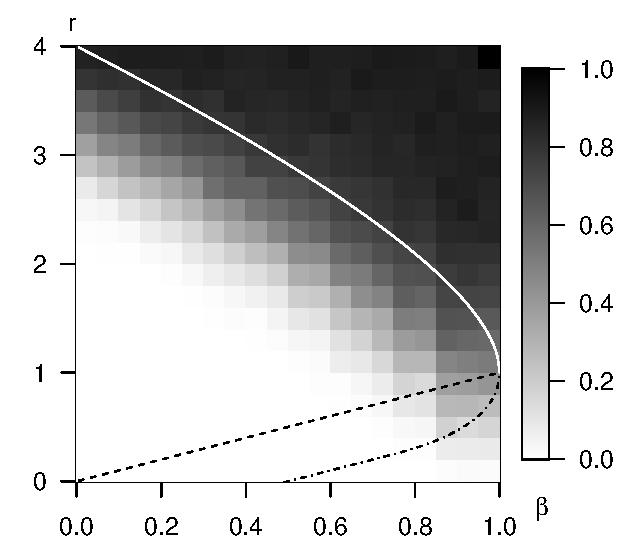
\includegraphics[width=0.4\textwidth]{./figures/simulated_phase_diagram_p100.eps}
      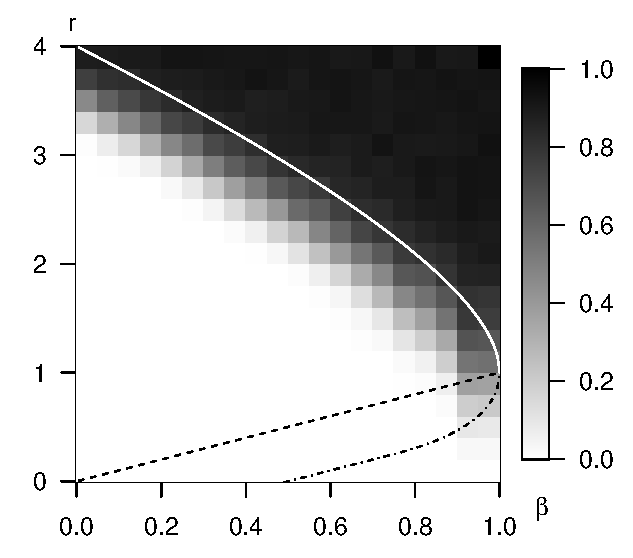
\includegraphics[width=0.4\textwidth]{./figures/simulated_phase_diagram_p10000.eps}
      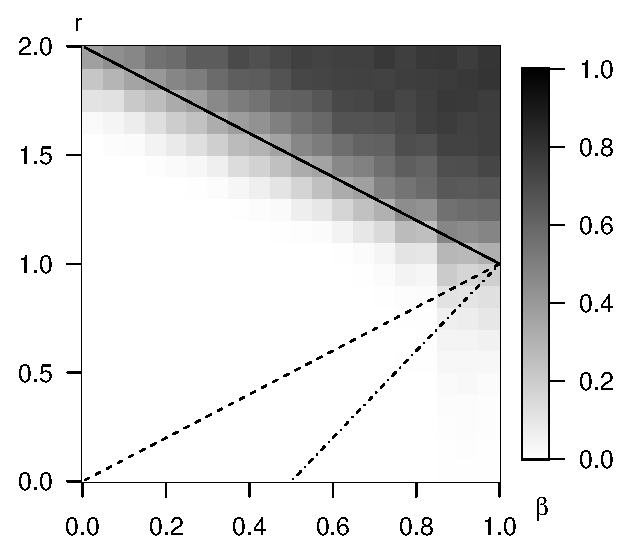
\includegraphics[width=0.4\textwidth]{./figures/simulated_phase_diagram_Laplace_p100_4.eps}
      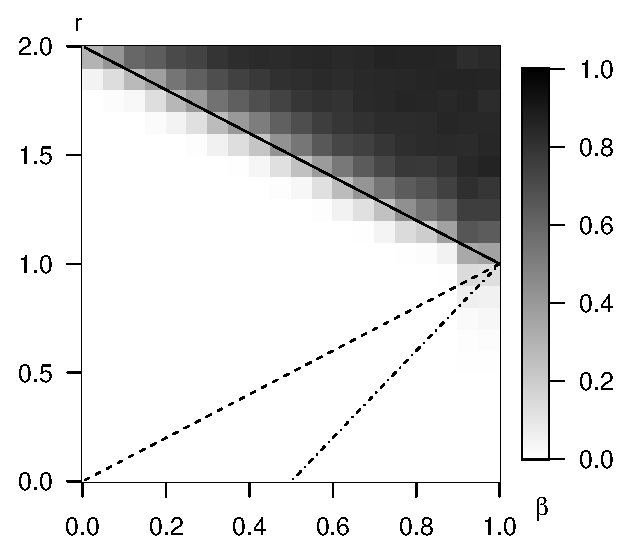
\includegraphics[width=0.4\textwidth]{./figures/simulated_phase_diagram_Laplace_p10000_4.eps}
      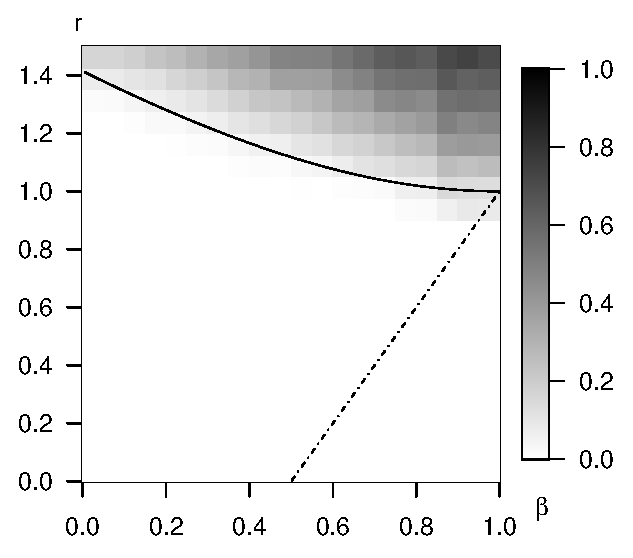
\includegraphics[width=0.4\textwidth]{./figures/simulated_phase_diagram_NLC_p100.eps}
      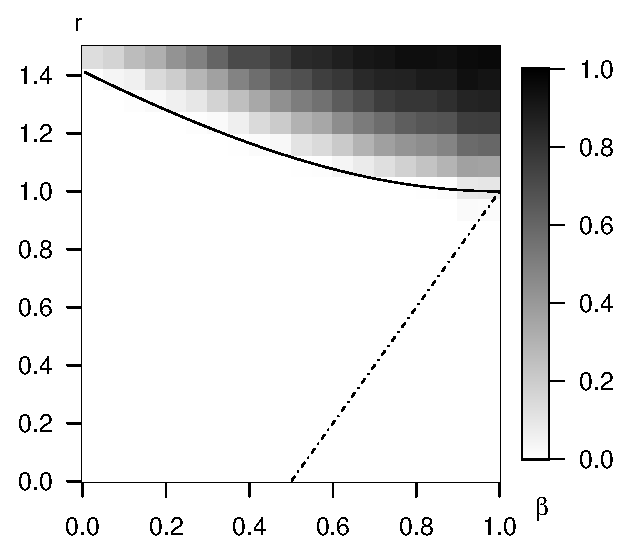
\includegraphics[width=0.4\textwidth]{./figures/simulated_phase_diagram_NLC_p10000.eps}
      \caption{The empirical probability of exact support recovery from numerical experiments, as a function of sparsity level $\beta$ and signal sizes $r$, 
      from Gaussian error models (upper panels), Laplace error models (middle panels), and generalized Gaussian with $\nu=1/2$ (lower panels); darker color indicates higher probability of exact support recovery. 
      The experiments were repeated 1000 times for each sparsity-signal size combination, and for dimensions $p=100$ (left panels) and $p=10000$ (right panels). 
      The numerical results agree with the boundaries described in Theorem \ref{thm:sufficient}. The convergence is noticeably slower for under the heavier 
      generalized Gaussian ($\nu=1/2$) errors.  For reference, the dashed and dash-dotted lines represent the weak classification and detection boundaries
       (see Chapter \ref{chap:phase-transitions}).
      \label{fig:phase-simulated}}
\end{figure}




We establish in this section minimax versions of our results from Section \ref{sec:boundary}.
Specifically, if we restrict ourselves to \emph{the class of thresholding procedures} $\cal T$ (defined in \eqref{eq:thresholding-procedure}), then Bonferroni's procedure is minimax optimal, for \emph{any} fixed dependence structures in the URS class.
This is formalized in Corollary \ref{cor:point-wise-minimax} in Section \ref{subsec:point-wise-minimax}.
We refer to this result as \emph{point-wise} minimax, to emphasize the fact that this optimality holds for every \emph{fixed} URS array.

Meanwhile, if we search over \emph{all procedures}, but expand the space of models to include {\em all} dependence structures, then a different minimax optimality statement holds for Bonferroni's procedure.
This result, formally stated in Section \ref{subsec:minimax-over-dependence}, is a consequence of our characterization of the finite-sample Bayes optimality of thresholding procedures in Sections \ref{subsec:Bayes-optimality} and \ref{subsec:optimal-procedure-sub-exponential}.
% The result is of independent interest and it is the main contribution of this section.

Finally, we offer some insights into the support recovery problem in the case when errors have heavier-than-exponential tails in Section \ref{subsec:optimal-procedure-super-exponential}.

\subsection{Point-wise minimax optimality}
\label{subsec:point-wise-minimax}

Theorems \ref{thm:sufficient} and \ref{thm:necessary} can be cast in the form of an asymptotic minimax statement. 
% (concealing the gap between sufficient and necessary conditions as pointed out in Remark \ref{rmk:gap-between-sufficient-necessary}).

\begin{corollary}[Point-wise minimax]
\label{cor:point-wise-minimax}
Let $\widehat{S}^{\text{Bonf}}$ be the sequence of Bonferroni's procedure described in Theorem \ref{thm:sufficient}. 
Let also the errors have common $\text{AGG}(\nu)$ distribution $F$ with parameter $\nu>0$, and $\Theta_p^+$ be as defined in \eqref{eq:minimax-signal-config-over}.
If $\underline{r}>g(\beta)$, then we have
\begin{equation} \label{eq:point-wise-minimax-above}
    \limsup_{p\to\infty} \sup_{\mu\in\Theta_p^+(\beta, \underline{r})} \P(\widehat{S}^{\text{Bonf}}_p \neq S_p) = 0,
\end{equation}
for arbitrary dependence structure of the error array ${\cal E} = \{\epsilon_p(i)\}_p$.
Let $\cal T$ be the class of thresholding procedures \eqref{eq:thresholding-procedure}. 
If $\underline{r}<g(\beta)$, then we have
\begin{equation} \label{eq:point-wise-minimax-below}
    \liminf_{p\to\infty} \inf_{\widehat{S}_p\in \cal T} \sup_{\mu\in\Theta_p^+(\beta, \underline{r})} \P(\widehat{S}_p \neq S_p) = 1,
\end{equation}
for any error dependence structure such that ${\cal E}\in U(F)$ and ${(-\cal E)}\in U(F)$.
\end{corollary}

\begin{proof}[Proof of Corollary \ref{cor:point-wise-minimax}]
The first conclusion \eqref{eq:point-wise-minimax-above} is a restatement of Theorem \ref{thm:sufficient}.

For the second statement \eqref{eq:point-wise-minimax-below}, since $\underline{r}<g(\beta)$, we can pick a sequence $\mu^*\in\Theta_p^+(\beta, \underline{r})$ such that $|S_p| = \lfloor p^{1-\beta}\rfloor$, with signals having the same signal size $\mu(i)=(2r\log{p})^{1/\nu}$ for all $i\in S_p$, where $\underline{r}<{r}<g(\beta)$.
For this particular choice of $\mu^*$ we have $\mu^*\in\Theta_p^-(\beta, \overline{r})$ where $r<\overline{r}<g(\beta)$,
and according to Theorem \ref{thm:necessary}, we obtain $\lim_{p\to\infty} \inf_{\widehat{S}_p\in \cal T} \mathbb P[\widehat{S}_p \neq S_p] = 1$, for all dependence structures in the URS class.
\end{proof}

\begin{remark}
Theorem \ref{thm:necessary} is a stronger result than the traditional minimax claim in Relation \eqref{eq:point-wise-minimax-below}.
Indeed,  \eqref{eq:classification-impossible-dependent} involves an infimum (over the class $\Theta^-_p$) while \eqref{eq:point-wise-minimax-below} has a supremum (over the class $\Theta^+_p$).

On the other hand, Corollary \ref{cor:point-wise-minimax} is more informative than many minimax-type statements, since it applies ``point-wise'' to any fixed error dependence structure in the URS class.
\end{remark}

\begin{remark}
Corollary \ref{cor:point-wise-minimax} echoes Remark \ref{rmk:dependence-assumptions}: for a very large class of dependence structures, we cannot improve upon Bonferroni's procedure in exact support recovery problems (asymptotically), unless we look beyond thresholding procedures.
% There is a limited amount of literature on non-thresholding procedures that utilize the error dependence structures to improve power.
% A notable effort was made by \citet{jin2014optimality}, where the performance (in terms of Hamming loss) of a so-called graphlet screening procedure was studied. 
\end{remark}

% This is an enhancement (in the asymptotic sense) of the minimax results in Section 4.1 of \cite{butucea2018variable}, where the supremum was taken over the dependence structures.






%\section{Bayes minimax optimality and (sub)optimality of thresholding procedures}


%\section{Strong classification boundaries in other light-tailed error models}
%\label{suppsec:other-boundaries}
%The strong classification boundaries extend beyond the AGG models.
As our analysis in Section \ref{sec:boundary} suggests, all additive error models where the errors have URS maxima demonstrate this phase transition phenomenon under appropriate parametrization of the sparsity and signal sizes.
We derive explicit boundaries for two additional classes of models under the general form of the additive noise models \eqref{eq:model-additive}, with heavier and lighter tails than the AGG models, respectively. 

We would like to point out that the sparsity and signal sizes can be re-parametrized for the boundaries to have different shapes.
For example in the case of Gaussian errors, if we re-parametrize sparsity $s$ with 
$\widetilde{\beta} = 2 - \left(1 + \sqrt{1-\beta}\right)^2$ where $\widetilde{\beta}\in(0,1)$, then the signal sparsity would have a slightly more complicated form:
$$
\left|S_p\right| = \left\lfloor p^{1-\beta} \right\rfloor = \left\lfloor p^{\left(\sqrt{2 - \widetilde{\beta}} - 1\right)^2}\right\rfloor,
$$
while the strong classification boundary would take on the simpler form:
\begin{equation}\label{eq:altenative-parametrization}
g(\beta) = \widetilde{g}(\widetilde{\beta}) = 2 - \widetilde{\beta}.
\end{equation}
In the next two classes of models we will adopt parametrizations such that the boundaries are of the form $\widetilde{g}$ in \eqref{eq:altenative-parametrization}.

\subsection{Additive error models with heavier-than-AGG tails}

Distributions such as the log-normal have heavier tails than the AGG model, yet the tails are nevertheless rapidly-varying. 
Therefore, Proposition \ref{prop:rapid-varying-tails} applies, and we expect to see phase-transition-type results when the additive errors have these heavier-than-AGG tails.

\begin{example}[Heavier than AGG] \label{exmp:heavier-than-AGG}
Let $\gamma>1$, $c>0$, and suppose that
\begin{equation} \label{eq:heavier-than-AGG}
    \log{\overline{F}(x)} = - \left(\log x\right)^\gamma \left(c+M(x)\right),
\end{equation}
where $\lim_{x\to\infty} M(x)\log^\gamma{x}= 0$. Then, Relation \eqref{eq:rapid-varying-tails} holds under 
model \eqref{eq:heavier-than-AGG}. Further, if the entries in the array are independent, the 
maxima are relatively stable.

The behavior of the quantiles $u_p$ in this model is as follows. As $p\to\infty,$
\begin{equation*}
    u_p \sim \exp{\left\{\left(c^{-1}\log{p}\right)^{1/\gamma}\right\}}
    \iff c\left(\log{u_p}\right)^{\gamma} + o(1) = \log(p) = - \log \overline{F}(u_p).
\end{equation*}
since $u_p$ diverges, and $M(u_p)$ is $o((\log^\gamma u_p)^{-1})$.
\end{example}


Following Example \ref{exmp:heavier-than-AGG}, assume that the errors in Model \eqref{eq:model-additive} have rapidly varying right tails
\begin{equation} \label{eq:heavier-than-AGG-boundary-1}
    \log{\overline{F}(x)} = - \left(\log x\right)^\gamma \left(c+M(x)\right),
\end{equation}
as $x\to \infty$, and left tails
\begin{equation} \label{eq:heavier-than-AGG-boundary-2}
    \log{{F}(x)} = - \left(\log{(-x)}\right)^\gamma \left(c+M(-x)\right),
\end{equation}
as $x\to -\infty$.

\begin{theorem} \label{thm:heavier-than-AGG}
Suppose the marginals $F$ follows \eqref{eq:heavier-than-AGG-boundary-1} and \eqref{eq:heavier-than-AGG-boundary-2}.
Let
$$
k(\beta) = \log{p} - \left((\log{p})^{1/\gamma} + \log{(1-\beta)}\right)^\gamma,
$$
and let the signal $\mu$ have 
$$|S_p| = \left\lfloor pe^{-k(\beta)} \right\rfloor$$
non-zero entries. Assume the magnitudes of non-zero signal entries are in the range between
$$\underline{\Delta} = \exp{\left\{(\log{p})^{1/\gamma}\right\}}\underline{r}
\quad\text{and}\quad
\overline{\Delta} = \exp{\left\{(\log{p})^{1/\gamma}\right\}}\overline{r}.$$
If $\underline{r} > \widetilde{g}(\beta) = 2 - \beta$, then Bonferroni's procedure $\widehat{S}_p$ (defined in \eqref{eq:Bonferroni-procedure}) with appropriately calibrated FWER $\alpha\to 0$ achieves asymptotic perfect support recovery, under arbitrary dependence of the errors.

On the other hand, when the errors are uniformly relatively stable, if $\overline{r} < \widetilde{g}(\beta) = 2 - \beta$, then no thresholding procedure can achieve asymptotic perfect support recovery with positive probability.
\end{theorem}


\subsection{Additive error models with lighter-than-AGG tails}


Similar to how Proposition \ref{prop:rapid-varying-tails} applies to models with heavier-than-AGG tails, it also to error models with lighter tails than the AGG class.

\begin{example}[Lighter than AGG] \label{exmp:lighter-than-AGG}
With $\nu>0$, and $L(x)$ a slowly varying function, the class of distributions
\begin{equation} \label{eq:lighter-than-AGG}
    \log{\overline{F}(x)} = - \exp{\left\{x^\nu L(x)\right\}},
\end{equation}
is rapidly varying.
The quantiles can be derived explicitly in a subclass of \eqref{eq:lighter-than-AGG} where $L(x)\to 1$, or equivalently, when $\log{|\log{\overline{F}(x)}|}\sim x^\nu$,
\begin{equation*}
    u_p \sim \left(\log \log{p}\right)^{1/\nu}
    \iff \exp{\left\{u_p^\nu\left(1+o(1)\right)\right\}} = \log(p) = - \log \overline{F}(u_p).
\end{equation*}
\end{example}
%The proofs of the rapid variation of the distributions in Examples \ref{exmp:heavier-than-AGG} and \ref{exmp:lighter-than-AGG} are entirely analogous to that of Example \ref{exmp:AGG}, and omitted.


Following Example \ref{exmp:lighter-than-AGG}, assume that errors in Model \eqref{eq:model-additive} has rapidly varying right tails
\begin{equation} \label{eq:lighter-than-AGG-boundary-1}
        \log{\overline{F}(x)} = - \exp{\left\{x^\nu L(x)\right\}},
\end{equation}
where $L(x)$ is a slowly varying function, as $x\to\infty$, and left tails
\begin{equation} \label{eq:lighter-than-AGG-boundary-2}
        \log{\overline{F}(x)} = - \exp{\left\{-x^\nu L(-x)\right\}},
\end{equation}
as $x\to -\infty$.

The phase transition results in multiple testing problems under such tail assumptions is characterizes as follows.

\begin{theorem} \label{thm:lighter-than-AGG}
Suppose marginals $F$ follow \eqref{eq:lighter-than-AGG-boundary-1} and \eqref{eq:lighter-than-AGG-boundary-2}.
Let
$$
k(\beta) = \log{p} - \left(\log(p)\right)^{(1-\beta)^\nu},
$$
and let the signal $\mu$ have 
$$|S_p| = \left\lfloor pe^{-k(\beta)} \right\rfloor$$
non-zero entries. Assume the magnitudes of non-zero signal entries are in the range between
$$\underline{\Delta} = \log{\log{p}}^{1/\nu}\underline{r}
\quad\text{and}\quad
\overline{\Delta} = \log{\log{p}}^{1/\nu}\overline{r}.$$
If $\underline{r} > \widetilde{g}(\beta) = 2 - \beta$, then Bonferroni's procedure $\widehat{S}_p$ (defined in \eqref{eq:Bonferroni-procedure}) with appropriately calibrated FWER $\alpha\to 0$ achieves asymptotic perfect support recovery, under arbitrary dependence of the errors.

On the other hand, when the errors are uniformly relatively stable, if $\overline{r} < \widetilde{g}(\beta) = 2 - \beta$, then no thresholding procedure can achieve asymptotic perfect support recovery with positive probability.
\end{theorem}





%\section{Thresholding procedures under heavy-tailed errors}
%\label{suppsec:heavy-tailed}
%We analyze the performance of thresholding estimators under heavy-tailed models in this section, and illustrate its lack of phase transition.
Suppose we have iid errors with Pareto tails in Model \eqref{eq:model-additive}, that is, $\epsilon(i)$'s have common marginal distribution $F$ where
\begin{equation} \label{eq:pareto-tails}
    \overline{F}(x) \sim x^{-\alpha} \quad \text{and} \quad F(-x) \sim x^{-\alpha},    
\end{equation}
as $x\to\infty$. 
It is well-known (see, e.g., Theorem 1.6.2 of \citep{leadbetter2012extremes}) that the maxima of iid Pareto random variables have Frechet-type limits.
Specifically, we have
\begin{equation} \label{eq:Frechet-limit-1}
    \frac{\max_{i\in\{1,\ldots,p\}}\epsilon(i)}{u_p} \implies Y,
\end{equation}
in distribution, where $u_p = F^{\leftarrow}(1-1/p)\sim p^{1/\alpha}$, and $Y$ is a standard $\alpha$-Frechet random variable, i.e.,
\begin{equation*}
    \P[Y\le t] = \exp{\{-t^{-\alpha}\}}, \quad t>0.
\end{equation*}
By symmetry in our assumptions, the same argument applies to the minima as well.

\begin{theorem} \label{thm:heavy-tails}
Let errors in Model \eqref{eq:model-additive} be as described in Relation \eqref{eq:pareto-tails}.
Let the signal have $s = |S| = fp$ non-zero entries, with magnitude $\Delta = rp^{1/\alpha}$, where both $f\in(0,1)$ and $r\in(0,+\infty)$ may depend on $p$, so that no generality is lost.

Under these assumptions, the necessary condition for thresholding procedures $\widehat{S}$ to achieve exact support recovery ($\P[\widehat{S}=S]\to1$) is 
\begin{equation} \label{eq:heavy-tails-exact-recovery}
    \liminf_{p\to\infty} r = \infty.
\end{equation}
Condition \eqref{eq:heavy-tails-exact-recovery} is also sufficient for the oracle thresholding procedure to succeed in the exact support recovery problem.

On the other hand, the necessary and sufficient condition for all thresholding procedures to fail exact support recovery ($\P[\widehat{S}=S]\to0$) is 
$$
\limsup_{p\to\infty} r = 0.
$$
\end{theorem}

In other words, Theorem \ref{thm:heavy-tails} states that there does not exist a non-trivial phase transition for thresholding procedures when errors have (two-sided) $\alpha$-Pareto tails.

\begin{proof}[Proof of Theorem \ref{thm:heavy-tails}]
Recall the oracle thresholding procedure $\widehat{S}^* = \left\{i:x(i) \ge x_{[s]}\right\}$, and the set of all thresholding procedures, denoted 
${\cal S}$ (see Definition \ref{eq:thresholding-procedure}).
The probability of exact support recovery by any thresholding procedure $\widehat{S}\in{\cal S}$ is bounded above by that of $\widehat{S}^*$, that is,
\begin{align}
    \max_{\widehat{S}\in{\cal S}}\P[\widehat{S}=S] 
        &= \P[\widehat{S}^*=S] 
        = \P\Big[\max_{i\in S^c}x(i) \le \min_{i\in S}x(i)\Big] \nonumber \\
        &= \P\Big[\frac{\max_{i\in S^c}x(i)}{u_p} \le \frac{\min_{i\in S}x(i)}{u_p}\Big] \nonumber \\
        &= \P\Big[\frac{M_{S^c}}{u_p} \le \frac{m_S}{u_p} + r_p\Big], \label{eq:heavy-tailed-case-proof-0}
        % &= \P\Big[\underbrace{(1-f)^{1/\alpha}Y^{(1)}}_{=:F_1} + \underbrace{f^{1/\alpha}Y^{(2)}}_{=:F_2} \le r\Big], 
\end{align}
where $M_{S^c} = \max_{i\in S^c}\epsilon(i)$ and $m_S = \min_{i\in S}\epsilon(i)$.
For any $\alpha > 0$, the following elementary relations hold,
\begin{equation*}
    0 < L \le (1-f)^{1/\alpha} + f^{1/\alpha} \le U < \infty, \quad \text{for all} \; f\in(0,1),
\end{equation*}
where $L = \min\left\{1, 2(1/2)^{1/\alpha}\right\}$ and $U = \max\left\{1, 2(1/2)^{1/\alpha}\right\}$.
Therefore we have,
\begin{equation} \label{eq:heavy-tailed-case-proof-1}
    U\max\left\{\frac{M_{S^c}}{u_p}, -\frac{m_S}{u_p}\right\} < r_p
    \implies
    (1-f)^{1/\alpha}\frac{M_{S^c}}{u_p} - f^{1/\alpha}\frac{m_S}{u_p} < r_p,
\end{equation}
and 
\begin{equation} \label{eq:heavy-tailed-case-proof-2}
    L\min\left\{\frac{M_{S^c}}{u_p}, -\frac{m_S}{u_p}\right\} < r_p
    \impliedby
    (1-f)^{1/\alpha}\frac{M_{S^c}}{u_p} - f^{1/\alpha}\frac{m_S}{u_p} < r_p.
\end{equation}
Putting together \eqref{eq:heavy-tailed-case-proof-0}, \eqref{eq:heavy-tailed-case-proof-1}, and \eqref{eq:heavy-tailed-case-proof-2}, we have
\begin{equation} \label{eq:heavy-tailed-case-proof-3}
    \P\Big[\max\left\{\frac{M_{S^c}}{u_p}, -\frac{m_S}{u_p}\right\} < r_p/U\Big]
    \le \P[\widehat{S}^*=S]
    \le \P\Big[\min\left\{\frac{M_{S^c}}{u_p}, -\frac{m_S}{u_p}\right\} < r_p/L\Big].
\end{equation}
We know from the weak convergence result \eqref{eq:Frechet-limit-1} that for any $\epsilon>0$ there is a constant $N$ such that for all $p>N$ we have 
\begin{equation} \label{eq:heavy-tailed-case-proof-3.5}
    \P\Big[\max\left\{\frac{M_{S^c}}{u_p}, -\frac{m_S}{u_p}\right\} < r_p/U\Big]
    \ge \P\Big[\max\left\{Y^{(1)}, Y^{(2)}\right\} < {r_p}/{U}\Big] - \epsilon,
\end{equation}
where $Y^{(1)}$ and $Y^{(2)}$ are independent $\alpha$-Frechet random variables with scale coefficients $(1-f)^{1/\alpha}$ and $f^{1/\alpha}$ respectively.
That is,
\begin{equation*}
    \P[Y^{(1)}\le t] = \exp{\{-(1-f)/t^\alpha\}}, 
    \quad \text{and} \quad
    \P[Y^{(2)}\le t] = \exp{\{-f/t^\alpha\}}.
\end{equation*}
Since the distributional limit in \eqref{eq:heavy-tailed-case-proof-3.5} has a density (with respect to the Lebesgue measure), we know that density is bounded above by a finite constant, say, $K$.
For the same choice of $\epsilon$ as before, we can find a further constant $N'$ such that for all $p>\max\{N, N'\}$ we have 
$$
    \liminf r_p < \epsilon/K + r_p,
$$
so that the right hand side of \eqref{eq:heavy-tailed-case-proof-3.5} is bounded by
\begin{equation} \label{eq:heavy-tailed-case-proof-3.6}
    \P\Big[\max\left\{Y^{(1)}, Y^{(2)}\right\} < {r_p}/{U}\Big] - \epsilon
    \ge \P\Big[\max\left\{Y^{(1)}, Y^{(2)}\right\} < \frac{\liminf r_p}{U}\Big] - 2\epsilon.
\end{equation}
By the arbitrariness in the choice of $\epsilon$, we conclude from \eqref{eq:heavy-tailed-case-proof-3.5} and \eqref{eq:heavy-tailed-case-proof-3.6} that
\begin{equation} \label{eq:heavy-tailed-case-proof-4}
    \liminf \P\Big[\max\left\{\frac{M_{S^c}}{u_p}, -\frac{m_S}{u_p}\right\} < r_p/U\Big]
    \ge \P\Big[\max\left\{Y^{(1)}, Y^{(2)}\right\} < \frac{\liminf r_p}{U}\Big].
\end{equation}
Combining Relations \eqref{eq:heavy-tailed-case-proof-3} and \eqref{eq:heavy-tailed-case-proof-4}, we know that if $\liminf r_p = \infty$, we must have 
$$
    \liminf\P\left[\widehat{S}^*=S\right]
    \ge \P\Big[\max\left\{Y^{(1)}, Y^{(2)}\right\} < \frac{\liminf r_p}{U}\Big] = 1.
$$
Conversely, if $\liminf\P\left[\widehat{S}^*=S\right]<1$, we must have $\liminf r_p < \infty$.

Similarly, we can obtain the upper bound of exact support recovery probability for the optimal thresholding procedure,
\begin{equation} \label{eq:heavy-tailed-case-proof-5}
    \limsup \P\Big[\min\left\{\frac{M_{S^c}}{u_p}, -\frac{m_S}{u_p}\right\} < r_p/L\Big]
    \le \P\Big[\min\left\{Y^{(1)}, Y^{(2)}\right\} < \frac{\limsup r_p}{L}\Big].
\end{equation}
The conclusions of the second part of Theorem \ref{thm:heavy-tails} follow from \eqref{eq:heavy-tailed-case-proof-3} and \eqref{eq:heavy-tailed-case-proof-5}.
\end{proof}

The probability of exact recovery can be approximated if the parameters $r$ and $f$ converge.
The next result follows from a small modification of the arguments in the proof of Theorem \ref{thm:heavy-tails}.

\begin{corollary}
Under the assumptions in Theorem \ref{thm:heavy-tails}, if 
$\lim r = r^*$, and $\lim f = f^*$, for some constant $r^*\ge0$ and $f^*\in[0,1]$, then 
$$
    \lim \P[\widehat{S}^*=S] 
    = \P\Big[(1-f^*)^{1/\alpha}Z_1 + (f^*)^{1/\alpha}Z_2 < {r^*}\Big].
$$
where $Z_1$ and $Z_2$ are independent standard $\alpha$-Frechet random variables, i.e., $\P[Z_i \le t] = \exp{\{-x^{-\alpha}\}}$, $x>0$.
\end{corollary}

\begin{remark}
Of course one might wonder if it would be meaningful to derive a ``phase transition'' under a different parametrization of the signal sizes, say 
\begin{equation} \label{eq:Pareto-parametrization-with-boundary}
    \Delta = p^{r/\alpha}.
\end{equation}
In this case, Theorem \ref{thm:heavy-tails} suggests that a ``phase transition'' takes place at $r=1$.
However, this non-multiplicative parametrization of the signal sizes would make power analysis (like in Example \ref{exmp:gap-when-signal-sparse}) dimension-dependent. 

To illustrate, in the case of Gaussian errors with variance 1, if we were interested in small signals of size $\sqrt{2r\log{p}}$, where $r<1$ is below the boundary \eqref{eq:strong-classification-boundary}, then we only need $n > 2/r$ samples to guarantee discovery of their support.
In the Pareto case with parametrization \eqref{eq:Pareto-parametrization-with-boundary}, however, if we were interested in small signals of size $p^{r/\alpha}$, where $r<1$, then the ``boundary'' says that we will need $n > p^{2(1-r)/\alpha}$ samples, which is exponential in the dimension $p$ and quickly diverges.
Recall that the ``boundary'' is really an asymptotic result in $p$. 
Such an approximation in finite dimensions becomes invalid.
\end{remark}




\section{Additional proofs}
\label{suppsec:proofs}
\subsection{Proof of the claims in Examples \ref{exmp:FWER-controlling_procedures} and \ref{exmp:signals-straddling-the-boundary}}
\label{subsec:proofs-examples}

\begin{proof}[Proof of claims in Example \ref{exmp:FWER-controlling_procedures}]
By the Mill's ratio for the standard Gaussian distribution,
$$
\frac{t_p \P\left[Z>t_p\right]}{\phi(t_p)} \to 1,\quad \text{as}\quad t_p\to\infty,
$$
where $Z\sim \text{N}(0,1)$. 
Using the expression for $t_p = \sqrt{2\log{p}}$, we have
$$
p \;\P\left[Z>t_p\right] \sim \sqrt{2\pi}^{-1}\left(2\log{p}\right)^{-1/2} \to 0,
$$
as desired. The rest of the claims follow from Corollary \ref{cor:FWER-controlling_procedures}.
\end{proof}


\begin{proof}[Proof of claims in Example \ref{exmp:signals-straddling-the-boundary}]
In the first scenario, signal sizes in $S^{(1)}_p$ are by definition above the strong classification boundary \eqref{eq:strong-classification-boundary}.
The signal in $S^{(2)}_p$ has size parameter $1+\delta<2-\beta<(1+\sqrt{1-\beta})^2$, and therefore falls below the boundary.

It remains to show that $\mathbb{P}[\widehat{S}^{\text{Bonf}}_p=S_p]\to 1$.
To do so, we define two new arrays 
$$
{\cal Y}^{(k)} = \{y^{(k)}_p(j),\;j=1,2,\ldots,p\},\quad k\in\{1,2\}_p,
$$
where $y^{(k)}_p(j)=x_p(j)$ if $j\not\in S^{(k)}_p$, and $y^{(k)}_p(j)=\widetilde{\epsilon}_p(j)$ if $j\in S^{(k)}_p$, using an independent error array $\{\widetilde{\epsilon}_p(j),\;j=1,\ldots,p\}$ with iid standard Gaussian elements.
That is, we replace the elements in $S^{(1)}_p$ and $S^{(2)}_p$ with iid standard Gaussian noise.
Notice both arrays ${\cal Y}^{(1)}$ and ${\cal Y}^{(2)}$ satisfy the conditions in Theorem \ref{thm:sufficient} (with sparsity parameter equal to $\beta$ and $1$, respectively). 
Hence, we have
$$
\P[\widehat{S}^{\text{Bonf}}_p\subseteq S_p] 
= \P\left[\max_{j\in S^c}x(j) \le t_p\right]
\le \P\left[\max_{j\in S^c}y^{(1)}(j) \le t_p\right] \to 0,
$$
and 
\begin{align*}
    \P[\widehat{S}^{\text{Bonf}}_p\supseteq S_p]
    &= \P\left[\min_{j\in S}x(j) > t_p\right] 
    \ge 1 - \P\left[\min_{j\in S^{(1)}}x(j) \le t_p\right] - \P\left[\min_{j\in S^{(2)}}x(j) \le t_p\right] \\
    &\ge 1 - \P\left[\min_{j\in S^{(1)}}y^{(2)}_p(j) \le t_p\right] - \P\left[\min_{j\in S^{(2)}}y^{(1)}_p(j) \le t_p\right] 
    \to 1,
\end{align*}
where $t_p$ is the threshold in Bonferroni's procedure. The conclusion follows.
% only need to show $\mathbb{P}[S^{(2)}_p\subseteq\widehat{S}^{\text{Bonf}}_p]\to 1$.

In the second scenario, the signal sizes in $S^{(2)}$ by definition falls below the strong classification boundary \eqref{eq:strong-classification-boundary}.
To see that no thresholding procedure succeeds, we adapt the proof of Theorem \ref{thm:necessary}.
In particular, we obtain
$$
    \P[\widehat{S}_p = S_p] 
    \le \P\left[\max_{j\in S^c}x(j) \le t_p < \min_{j\in S}x(j)\right]
    \le \P\left[\max_{j\in S^c}x(j) < \min_{j\in S^{(2)}}x(j)\right].
$$
By the assumption that signals in $S^{(2)}$ have size parameter $(1-\delta)g(\beta)$, we have
\begin{equation}
\P\left[\max_{j\in S^c}x(j) < \min_{j\in S^{(2)}}x(j)\right]
= \P\left[ \frac{M_{S^{c}}}{u_p} < \frac{\sqrt{2(1-\delta)g(\beta)\log{p}} - m_{S^{(2)}}}{u_p}\right], 
\end{equation}
where $M_{S^{c}} = \max_{j\in S^{c}}\epsilon(j)$ and $m_{S^{(2)}} = \max_{j\in S^{(2)}}\left(-\epsilon(j)\right)$.
The ratio on the left-hand-side of the inequality converges to 1 as in \eqref{eq:classification-possible-dependent-proof-3} in the main text, whereas the term on the right-hand-side
\begin{align*}
    \frac{\sqrt{2(1-\delta)g(\beta)\log{p}} - m_{S^{(2)}}}{u_p} 
    &= \sqrt{(1-\delta)g(\beta)} - \frac{m_{S^{(2)}}}{u_{|S^{(2)}|}} \frac{u_{|S^{(2)}|}}{u_p} \\
    &\xrightarrow{\P} \sqrt{(1-\delta)} + \sqrt{1-\beta}(\sqrt{(1-\delta)} - 1) < 1.
\end{align*}
where we used the URS of the error arrays, and that 
$$
u_{|S^{(2)}|} \sim \sqrt{2\log{(p^{1-\beta}/2)}} 
= \sqrt{2(({1-\beta})\log{p}-\log2)} \sim \sqrt{2({1-\beta})\log{p}}.
$$
to conclude the convergence in probability.
\end{proof}









